%% abtex2-modelo-livro.tex, v<VERSION> ycherem
%% Copyright 2012-2013 by abnTeX2 group at http://abntex2.googlecode.com/
%%
%% This work may be distributed and/or modified under the
%% conditions of the LaTeX Project Public License, either version 1.3
%% of this license or (at your option) any later version.
%% The latest version of this license is in
%%   http://www.latex-project.org/lppl.txt
%% and version 1.3 or later is part of all distributions of LaTeX
%% version 2005/12/01 or later.
%%
%% This work has the LPPL maintenance status `maintained'.
%%
%% The Current Maintainer of this work is 
%% Youssef Cherem <ycherem@gmail.com>, member of abnTeX2 team, 
%% led by Lauro César Araujo. Further information are available on 
%% http://abntex2.googlecode.com/
%%
%% This work consists of the files abtex2-modelo-glossarios.tex,
%% abntex2-modelo-include-comandos and abntex2-modelo-references.bib
%%


\documentclass[
	% -- opções da classe memoir --
	10pt,				% tamanho da fonte
	openright,			% capítulos começam em pág ímpar (insere página vazia caso preciso)
	twoside,			% para impressão em verso e anverso. Oposto a oneside
	a5paper,			% tamanho do papel. 
	% -- opções da classe abntex2 --
	%chapter=TITLE,		% títulos de capítulos convertidos em letras maiúsculas
	%section=TITLE,		% títulos de seções convertidos em letras maiúsculas
	%subsection=TITLE,	% títulos de subseções convertidos em letras maiúsculas
	%subsubsection=TITLE,% títulos de subsubseções convertidos em letras maiúsculas
	% -- opções do pacote babel --
	english,			% idioma adicional para hifenização
	french,				% idioma adicional para hifenização
	spanish,			% idioma adicional para hifenização
	brazil,				% o último idioma é o principal do documento
]{abntex2}

% compilação de fontes

\usepackage{ifxetex}
\ifxetex
% % se for utilizar as fontes do sistema: **escolha sua fonte**
 \usepackage{polyglossia}
\setmainlanguage{brazil}
\setotherlanguages{french,english,spanish,german,italian}
\usepackage{fontspec}
\defaultfontfeatures{Ligatures=TeX}
\setmainfont[Numbers=OldStyle]{Minion Pro} %fonte principal (serifada)
\setsansfont[Scale=0.9]{Myriad Pro} %fonte sem serifas
\setmonofont[Scale=MatchLowercase]{Consolas} % fonte monoespaçada
 % comandos de fontes
\else
 % % se for utilizar pdflatex
 \usepackage[utf8]{inputenc}
 \usepackage[T1]{fontenc}
 \usepackage[american,frenchb,spanish,brazil]{babel}
 \usepackage{ebgaramond}
\fi
%% Observação: o pacote polyglossia pode apresentar erro ao ser utilizado com ifxetex + babel. 
%% Se isso acontecer, atualize o pacote para a versão mais recente ou utilize somente uma das sequências (pdflatex ou xelatex), comentando ou apagando a outra.

\usepackage[dvipsnames]{xcolor} 	% para cores
\usepackage{graphicx} 				% para imagens
\usepackage{booktabs,tabularx,rotating}% para tabelas
\usepackage{lipsum} 				% para texto de preenchimento de exemplo
\usepackage{mdframed} 				% para caixas de texto como na CIP do verso do título
\usepackage{microtype} 				% para melhorias de justificação
\usepackage{multicol}				% tabelas com colunas mescladas
\usepackage[alf]{abntex2cite} 		% pacote de citações
\usepackage{lettrine}				% 
\usepackage{xspace} 				% para nao precisar de espaços com {} depois de comandos
									% como \LaTeX e abreviações criadas pelo usuário

% ---
% Informações do documento
% ---
\title{Exemplo de livro}
\author{Youssef Cherem}
\date{2013}

% informações do PDF
\makeatletter
\hypersetup{
     	%pagebackref=true,
		pdftitle={\@title}, 
		pdfauthor={\@author},
    	pdfsubject={Breve sinopse do documento},
	    pdfcreator={LaTeX with abnTeX2},
		pdfkeywords={abnt}{latex}{abntex}{abntex2}{livro}, 
		colorlinks=true,       		% false: boxed links; true: colored links
    	linkcolor=blue,          	% color of internal links
    	citecolor=blue,        		% color of links to bibliography
    	filecolor=magenta,      		% color of file links
		urlcolor=blue,
		bookmarksdepth=4
}
\makeatother
% ---

% ---
% Estilo de capítulos
%
% \chapterstyle{pedersen} 
% \chapterstyle{lyhne} 
% \chapterstyle{madsen} 
\chapterstyle{veelo} 
%
% Veja outros estilos em:
% http://www.tex.ac.uk/tex-archive/info/MemoirChapStyles/MemoirChapStyles.pdf
% ---

% para cabeçalhos sem estar em maiúsculas
\nouppercaseheads 

% ---
% Espaçamentos entre linhas e parágrafos
% ---
% O tamanho do parágrafo é dado por:
%\setlength{\parindent}{1.3cm}
 
% Controle do espaçamento entre um parágrafo e outro:
%\setlength{\parskip}{0.2cm}  % tente também \onelineskip

% Margens do documento
%\setlrmarginsandblock{3cm}{2cm}{*}
%\setulmarginsandblock{3cm}{2cm}{*}
%\checkandfixthelayout
% ---


% ---
% Início do documento
% ---
\begin{document}
\frenchspacing

% ---
% Capa principal
% ---
\frontmatter

\begin{titlingpage}

\phantom{xxx}
\vspace{0.5cm}
\huge
\raggedright
Fulano de Tal\\
\vspace{2.5cm}
\Huge 
{\raggedleft
\textit{\textcolor{red}{Exemplo de livro composto com}} \LaTeX\\[1cm]
}
\centering 
%  %este é um símbolo que só aparecerá com a fonte Minion.
\vfill
\Large
% %este é um símbolo que só aparecerá com a fonte Minion.
Publicações Acadêmicas, Ltda.

\end{titlingpage}
% ---

% ---
% Contra-capa
% ---
\begin{titlingpage}

\phantom{xxx}
\vspace{0.5cm}
\huge
\raggedright
Fulano de Tal\\
\vspace{2.5cm}
\Huge 
{\raggedleft
\textit{\textcolor{red}{Exemplo de livro composto com}} \LaTeX\\[1cm]
}
\centering 
% %este é um símbolo que só aparecerá com a fonte Minion.
\vfill
\Large
% %este é um símbolo que só aparecerá com a fonte Minion.
Publicações Acadêmicas, Ltda.
% ---

% ---
% Verso da contra-capa
% ---
\clearpage
\footnotesize
%\raggedright
© 2013 Fulano de Tal \& Publicações Acadêmicas, Ltda.
%este é só um exemplo de copyright.

Qualquer parte desta publicação pode ser reproduzida, desde que citada a fonte.

\bigskip

\begin{center}
Dados Internacionais de Catalogação na Publicação (\textsc{cip})
Câmara Brasileira do Livro, \textsc{sp}, Brasil
\end{center}

\begin{mdframed}
\noindent Tal, Fulano de.

Exemplo de livro composto com \LaTeX. / Fulano de Tal. -- São Paulo: Publicações Acadêmicas, Ltda., 2013.

\medskip

Bibliografia.

ISBN XXXX-XXXX-XX.

\medskip

1. Programas de computador. 2. Tipografia. 3. Latex. 4. Normas ABNT.

\end{mdframed}

\end{titlingpage}
% ---


% ---
% inserir lista de ilustrações
% ---
\pdfbookmark[0]{\listfigurename}{lof}
\listoffigures*
\cleardoublepage

% ---
% inserir lista de tabelas
% ---
\pdfbookmark[0]{\listtablename}{lot}
\listoftables*
\cleardoublepage
% ---

% ---
% inserir o sumario
% ---
\pdfbookmark[0]{\contentsname}{toc}
\tableofcontents*
\cleardoublepage
% ---


\mainmatter

% ------------------------------------------------------------
\chapter*{Introdução}
% ------------------------------------------------------------

\lettrine[nindent=0.35em,lhang=0.40,loversize=0.3]{E}{ste documento} faz parte
do projeto ABN\TeX, destinando-se a servir como modelo para composição e
diagramação de livros em \LaTeX. Ele foi concebido para servir de base para
elaboração de livros baseados na norma NBR 6029:2006 da \textsc{abnt}, para
livros. Essa norma não estabelece parâmetros tão rígidos quanto a NBR
14724:2011, para trabalhos acadêmicos, e segue, de certa forma, o design usual
de livros. (Para facilitação da compreensão de termos técnicos, ver a Tabela
\ref{vocabulario-texto} com alguns termos do design de livros.)

Desta forma, temos:

\begin{description}
\item[parte pré-textual] Composta por: falsa folha de rosto, folha de rosto,
colofão (opcional na parte pós-textual), sumário (conteúdo),
a\-gra\-de\-ci\-men\-tos (acknowledgments), dedicatória, epígrafe.
\item[folha de rosto] Como diz o nome em inglês (\textit{title page}) a “folha
de rosto” é a \textit{página do título}. No verso da folha de rosto, costuma-se
incluir os dados sobre a obra e a edição, catalogação, editora, direitos
autorais e de reprodução etc.
\item [parte pós-textual] Composta por epílogo, posfácio, apêndice, glossário,
bibliografia, índice remissivo (inglês: \textit{index}), colofão etc.

\end{description}

Este modelo foi composto com a classe \texttt{memoir}, mas qualquer outra classe que contemple o formato de livros poderia ser utilizada. A formatação de geral dos capítulos, margens, tamanho de página, fontes etc. pode ser modificada pelo usuário.

% ------------------------------------------------------------
\chapter{Um exemplo de capítulo}
% ------------------------------------------------------------

\lipsum[1-10]

% ------------------------------------------------------------
\chapter{Exemplos de imagens}
% ------------------------------------------------------------

\lipsum[1-5]

\begin{figure}
\centering
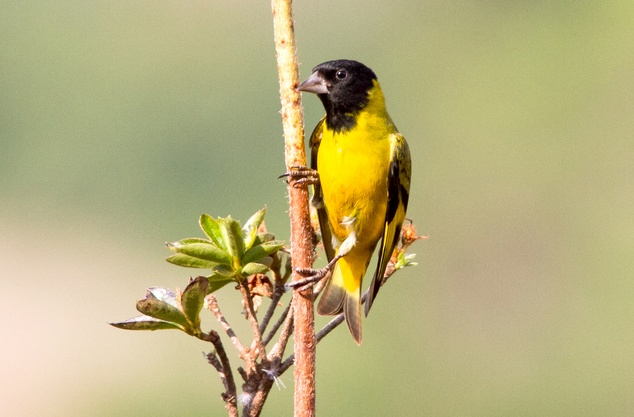
\includegraphics[width=0.6\linewidth]{pintassilgo}
\caption{Pintassilgo (\textit{Carduelis magellanicus}).}
\label{fig:pintassilgo}
\end{figure}


\begin{figure}
\centering
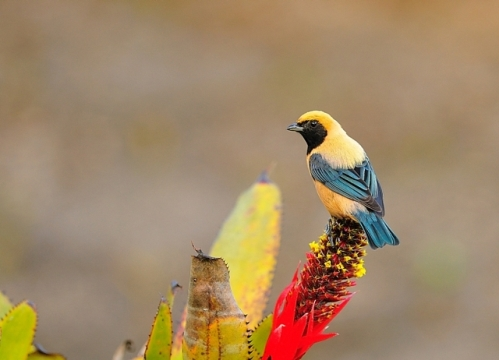
\includegraphics[width=0.6\linewidth]{saira-amarela}
\caption{Saíra-amarela (\textit{Tangara cayana}).}
\label{fig:saira-amarela}
\end{figure}

\begin{figure}
\centering
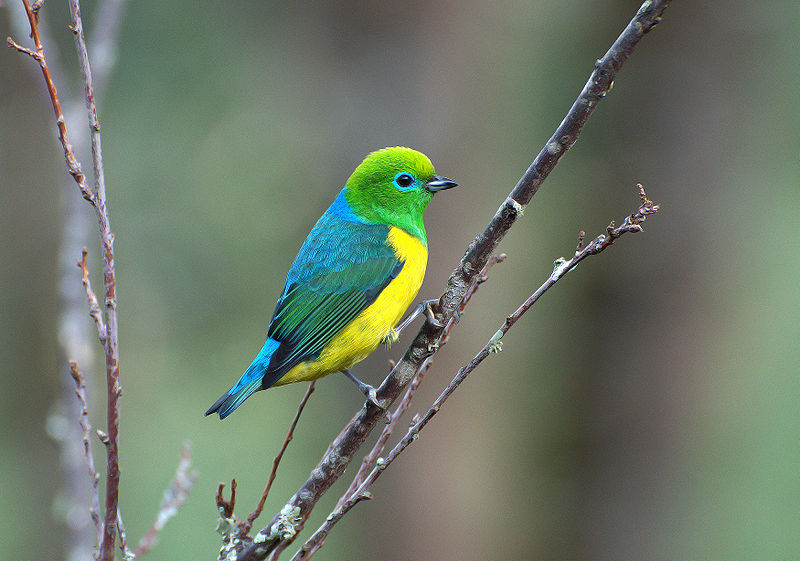
\includegraphics[width=0.6\linewidth]{bandeirinha}
\caption{Bandeirinha (\textit{Chlorophonia cyanea}).}
\label{fig:bandeirinha}
\end{figure}




% ------------------------------------------------------------
\chapter{Um exemplo de capítulo}
% ------------------------------------------------------------

\section{Exemplos de tabela}



\begin{table}
\caption{Pequeno vocabulário de design de livros\label{vocabulario-texto}}
\footnotesize
\begin{tabular}{p{5cm}p{5cm}}
\toprule
\textit{Termo em inglês} & \textit{Termo em português}\\
\midrule
\footnotesize
title page & folha de rosto.\\

cover & capa\\

back cover & quarta capa ou contra-capa ou verso da capa\\

bastard title ou half title & falsa folha de rosto. Tem só o título do livro.\\

table of contents & sumário\\

text block ou book block & miolo\\

print space (alemão: \textit{Satzspiegel}) & mancha gráfica\\

section, gathering, quire (especialmente se não impresso), signature & caderno\\

leaf = folio (latim) & folha, composta de recto (lat.) (anverso/frente) e verso (lat.) (verso). Geralmente o recto é página ímpar, e verso é página par.\\

hardcover & capa dura.\\

endpaper/endsheet & folha de guarda. Folha de papel para prender o miolo do livro na capa dura.\\

dust jacket, dust cover, book jacket, dust wrapper & sobrecapa. Geralmente de papel, para cobrir capas duras.\\

front matter & parte pré-textual.\\

main matter & parte textual\\

back matter & parte pós-textual. Composta por epílogo, posfácio, apêndice, glossário, bibliografia, índice remissivo (inglês: index), colofão etc.\\

colophon & colofão. Breve descrição sobre aspectos da publicação do livro. \\

running headers & títulos correntes\\

volume & volume. Conjunto de páginas encadernadas.\\

\bottomrule
\end{tabular}
\caption*{\footnotesize Fontes:\\
\url{http://pt.wikipedia.org/wiki/Design_de_livros}\\
\url{http://en.wikipedia.org/wiki/Book_design}\\
\url{http://static.lexicool.com/dictionary/RX7KW614433.pdf}\\}
\end{table}


\begin{table}
\caption{Exemplo de tabela utilizando o pacote \textsf{booktabs}.}
\centering
\begin{tabular}{llr}
\toprule
\multicolumn{2}{c}{Item} \\
\cmidrule(r){1-2}
Animal    & Description & Price (\$) \\
\midrule
Gnat      & per gram    & 13.65      \\
          & each        & 0.01       \\
Gnu       & stuffed     & 92.50      \\
Emu       & stuffed     & 33.33      \\
Armadillo & frozen      & 8.99       \\
\bottomrule
\multicolumn{3}{l}{\footnotesize Fonte: \url{http://en.wikibooks.org/wiki/LaTeX/Tables}}
\end{tabular}
\end{table}

% ------------------------------------------------------------
\chapter{Exemplos de citação}
% ------------------------------------------------------------

Uma citação de Fulano: \citeonline{fulano}.

\cite{fulano}.


\bibliography{modelo-livro} % insere o arquivo de bibliografia (.bib)

\backmatter % pós-textual

% ------------------------------------------------------------
% para última página com informações sobre a composição do livro.
\cleardoublepage
\thispagestyle{empty} 

Sinta-se convidado a participar do projeto ABN\TeX! Acesse o site do projeto em
\url{http://abntex2.googlecode.com/}. Também fique livre para conhecer, estudar,
alterar e redistribuir o trabalho do ABN\TeX, desde que os arquivos modificados
tenham seus nomes alterados e que os créditos sejam dados aos autores originais,
nos termos da ``The \LaTeX\ Project Public
License''\footnote{\url{http://www.latex-project.org/lppl.txt}}.

Encorajamos que sejam realizadas customizações específicas deste exemplo para
universidades e outras instituições --- como capas, folhas de rosto, etc.
% ~\vfill Este texto foi composto em Minion Pro, de Robert Slimbach, e Myriad Pro,
% de Robert Slimbach e Carol Twombly.
~\vfill Este texto foi composto em fontes EBGaramond
(\url{http://www.ctan.org/tex-archive/fonts/ebgaramond}).

\end{document}